\section{Experiments}
\label{sec:experiments}

In the following sections, we present the results of our experiments. We begin by examining the variability and bias in the estimates of the regression coefficients. We then move on to predictive performance and hyperparameter selection. We also consider the effect of class imbalance on the estimates of the regression coefficients. Finally, we look at the effect of interactions between features on the estimates of the regression coefficients.

In all cases where we use simulated data, we generate our response vector according to
\[
  \vec{y} = \mat{X}\vec{\beta}^* + \vec{\varepsilon},
\]
with \(\vec{\varepsilon} \sim \normal(\vec{0}, \sigma_\varepsilon^2 \mat{I})\), where \(\mat{X}\) is the design matrix, \(\vec{\beta}^*\) is the vector of true regression coefficients, and \(\sigma_\varepsilon^2\) is the noise level.

We consider two types of features: binary and quasi-normal features.
To generate binary vectors, we sample \(\ceil{qn}\) indexes uniformly at random without replacement from \(\{1,2,\dots,n\}\) and set the corresponding elements to one and the remaining ones to zero.
To generate quasi-normal features, we generate a linear sequence \(\vec{w}\) with \(n\) values from  \(10^{-4}\) to \(1 - 10^{-4}\), and set
\[
  x_{ij} = \cdf^{-1}(w_i)
\]
and then shuffle the elements of \(\vec{x}_j\) uniformly at random.

In each case, we fit either the lasso (the elastic net with \(\lambda_1 = \alpha \lambda\) ) or ridge (the elastic net with \(\lambda_2 = (1 - \alpha)\lambda\)). To normalize the data, we use
standardization for all quasi-normally distributed features and otherwise
\[
  s_j = (q - q^2)^\delta,
\]
which is equivalent to the (uncorrected) sample variance raised to the power of \(\delta\).

Throughout the experiments, we have used the \pkg{Lasso.jl} package~\citep{kornblith2024} to fit lasso or ridge regression, which implements the coordinate descent algorithm by citet{friedman2010}. All experiments were coded using the Julia programming language~\citep{bezanson2017} and the code is availabe at \url{https://github.com/jolars/normreg}.

\subsection{Variability and Bias in Estimates}\label{sec:experiments-varbias}

In our first experiment, we consider fitting the lasso to a simulated data set with \(n=500\) observations and \(p = \num{1000}\) features, out of which the first 20 features correspond to signals, with \(\beta_j^*\) decreasing linearly from 1 to 0.1.
We introduce dependence between the features by copying the first \(\ceil{\rho n/2}\) values from the first feature to each of the following features.
In addition, we set the class balance of the first 20 features so that it decreases linearly on a log-scale from 0.5 to 0.99.
We estimate the regression coefficients using the lasso, setting \(\lambda_1 = 2 \sigma_\varepsilon \sqrt{2 \log p }\) and compare the estimates to the true coefficients. We run the experiment for 50 iterations in each case and aggregate the results by reporting means and standard deviations.

The results~(\Cref{fig:binary-decreasing}) show that there is a considerable effect of class balance, particularly in the case of no scaling (\(\delta = 0\)), which corroborates our theoretical results from \Cref{sec:theory-binary-features}. At \(q=0.99\), for instance, the estimate (\(\hat{\beta}_{20}\)) is consistently zero when \(\delta = 0\). There is a similar effect also in the case of standardization (\(\delta = 1/2\)), but it is less pronounced. For \(\delta=1\) (variance scaling), we see that the effect of class balance on the estimates is, if anything, the reverse when the class imbalance is severe. What is also clear is that the variance of the estimates increase with class imbalance and that this effect increases together with \(\delta\). The level of correlation between the features introduces additional variance in the estimates but also seems to increase the effect of class imbalance in the cases when \(\delta = 0\) or \(1/2\).

\begin{figure}[htpb]
  \centering
  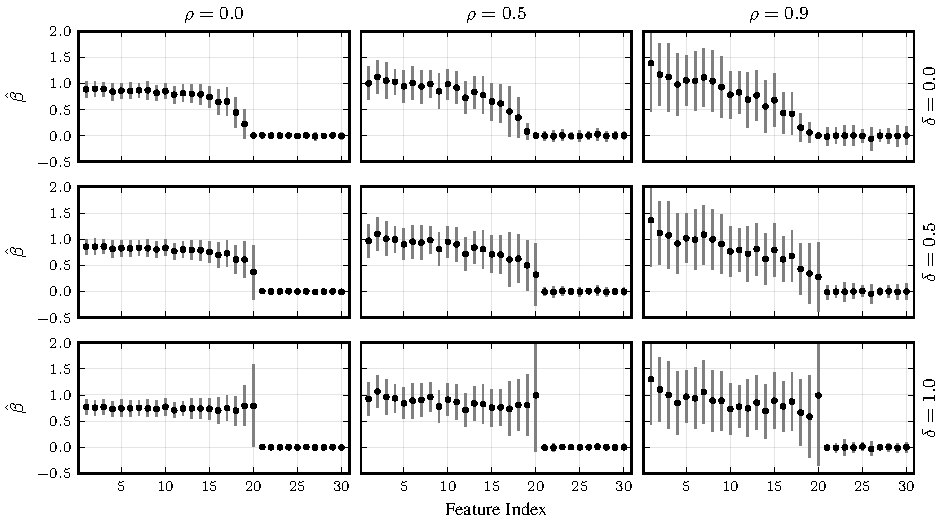
\includegraphics[]{plots/binary_decreasing.pdf}
  \caption{%
    Estimates of the regression coefficients from the lasso, \(\hat{\vec{\beta}}\), for the first 30 coefficients in the experiment. All of the features are binary and the first 20 features correspond to true signals with \(\beta_j^* = 2\) and geometrically decreasing class balance from 0.5 to 0.99. The remaining features have a class balance \(q_j \in [0.5, 0.99]\), distributed linearly among the features. The plot shows means and standard deviations averaged over 50 iterations.}
  \label{fig:binary-decreasing}
\end{figure}

\subsection{Predictive Performance}\label{sec:predictive-performance}

In this experiment, we consider predictive performance in terms of mean-squared error of the lasso given different levels of class balance (\(q \in \{0.5, 0.9, 0.99\}\)), signal-to-noise ratio, and normalization (\(\delta\)). As in the previous section, all of the features are binary, but here we have used \(n=300\), \(p = \num{1000}\). The \(k=10\) first features correspond to true signals with \(\beta^*_j = 1\) and all have class balance \(q\). To set signal-to-noise ratio levels, we rely on the same choice as in \citet{hastie2020} and use a log-spaced sequence of values from 0.05 to 6.

To estimate prediction performance, we use a standard hold-out validation method equal splits for the training, validation, and test sets. We fit a full lasso path, parameterized by a log-spaced grid of 100 values\footnote{This is a standard choice of grid, used for instance by \citet{friedman2010}}, from \(\lambda_\text{max}\) (the value of \(\lambda\) at which the first feature enters the model) to \(10^{-2}\lambda_\text{max}\) on the training set and pick a \(\lambda\) based on validation set error. Then we compute the hold-out test set error and aggregate the results across 100 iterations.

The results~(\Cref{fig:binary-sim}) show that the optimal normalization type in terms of prediction power depends on the class balance of the true signals. If the imbalance is severe, then we gain from using \(\delta=1/2\) or \(1\), which gives a chance of recovering the true signals. If everything is balanced, however, then we do better by not scaling at all. In general, \(\delta=1/2\) works well for these specific combinations of settings.

\begin{figure}[htpb]
  \centering
  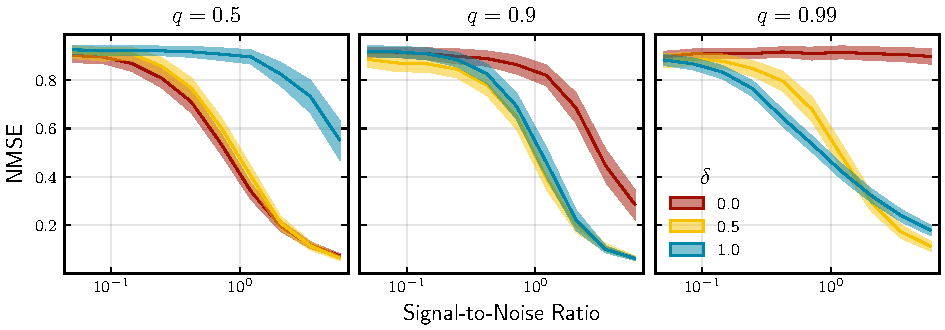
\includegraphics[]{plots/binary_data_sim.pdf}
  \caption{%
    Normalized mean-squared prediction error in a lasso model for different types of normalization (\(\delta\)), types of class imbalances (\(q\)), and signal-to-noise ratios (0.05 to 6) in a data set with \(n=300\) observations and \(p = \num{1000}\) features. The error is aggregated test-set error from hold-out validation with \(100\) observations in each of the training, validation, and test sets. The plot shows means and Student's \(t\)-based 95\% confidence intervals.
  }
  \label{fig:binary-sim}
\end{figure}

\subsection{Normalization as a Hyperparameter}\label{sec:experiments-hyperparameter}

% TODO: consider reparameterizing with respect to lambda/delta

Our previous results (particularly those from \Cref{sec:predictive-performance}) suggest that the choice of normalization matters for predictive performance. These results have relied on knowledge of the measurement error (signal-to-noise ratio), which we do not have reliable estimates of in practice (at least not in the high-dimensional context). An alterative that, however, comes naturally as a consequence of our particular parameterization using \(\delta\), is to treat the choice of normalization as a hyperparameter and optimize over it. This is the approach we take in this experiment.

We set up a grid of \(\lambda\) values as in \Cref{sec:predictive-performance} and, in addition, also create a linearly spaced grid of \(\delta\) values in \([0, 1]\). We split the data into a 50/50 training/validation set split and for each point in this two-dimensional grid fit the lasso or ridge to the training set and compute a hold-out validation set error. We do this for three data sets: \data{a1a}~\citep{becker1996}, \data{rhee2006}~\citep{rhee2006}, and \data{w1a}~\citep{platt1998}.

\begin{table}[hbtp]
  \centering
  \caption{Details of the real datasets used in the experiments}
  \begin{tabular}{lS[table-format=4.0]S[table-format=3.0]l}
    \toprule
    Dataset         & {\(n\)} & {\(p\)} & {Response} \\
    \midrule
    \data{w1a}      & 2477    & 300     & Binary     \\
    \data{a1a}      & 1605    & 123     & Binary     \\
    \data{rhee2006} & 842     & 361     & Continuous \\
    \bottomrule
  \end{tabular}
\end{table}

We show estimated level-curves of validation set error, in terms of normalized mean-squared error (NMSE), in \Cref{fig:hyperopt-contours}. For \data{a1a}, the lasso is generally quite insensitive to the type of normalization, even if the optimal value is around 0.2. For ridge regression, lower values of \(\delta\) clearly work better. With the \data{w1a} data set, however, the relationship is flipped in the case of ridge regression and the optimal value is approximately 0.8. In the case of the lasso (for \(\data{w1a}\)), a value around 0.5 is optimal and low values (little scaling) yield worse prediction errors. Finally, for \data{rhee2006}, the lasso is again insensitive to normalization type. This is not the case for ridge, however, where a value around 0.2 is optimal and high values of \(\delta\) yield worse prediction errors.

\begin{figure}[htpb]
  \centering
  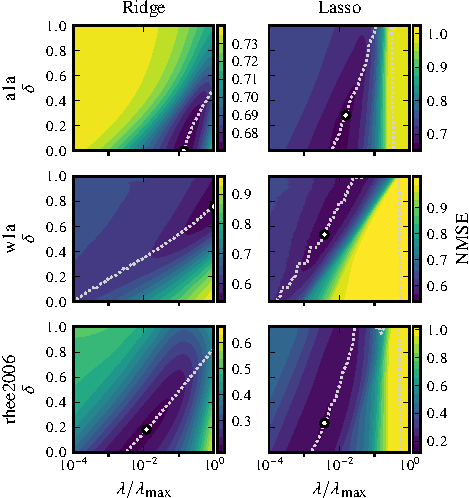
\includegraphics[]{plots/hyperopt_surfaces.pdf}
  \caption{%
    Contour plots of normalized mean-squared error (NMSE) for the hold-out validation set across a grid of \(\delta\) and \(\lambda\) values for ridge regression and the lasso. The dotted path shows the smallest NMSE as a function of \(\lambda\). The dot marks the combination with the smallest error.
  }
  \label{fig:hyperopt-contours}
\end{figure}

We would like to point out that there is a dependency between \(\lambda\) and \(\delta\) here that make it difficult to interpret the relationship between them and the error. This comes fro mthe fact that scaling with a smaller value (as in \(\delta = 1\)) increases the sizes of the vectors, which means that the level of penalization is relaxed, relative speaking.

In \Cref{fig:hyperopt-support}, we have, in addition to NMSE on the validation set, also plotted the size of the support of the lasso (cardinality of the set of features that have corresponding nonzero coefficients). Here, however, we only show results for \(\delta \in \{0, 1/2, 1\}\). It is clear that \(\delta = 1/2\) works quite well for all of these three data sets, being able to attain a value close to the mininum for each of the three data sets. This is not the case for \(\delta \in \{0, 1\}\), for which the best possible prediction error is considerably worse. This is particularly the case with \(\delta =0\) and the \data{w1a} data set. The dependency between \(\lambda\) and \(\delta\) is also visible here by looking at the support size.

\begin{figure}[htpb]
  \centering
  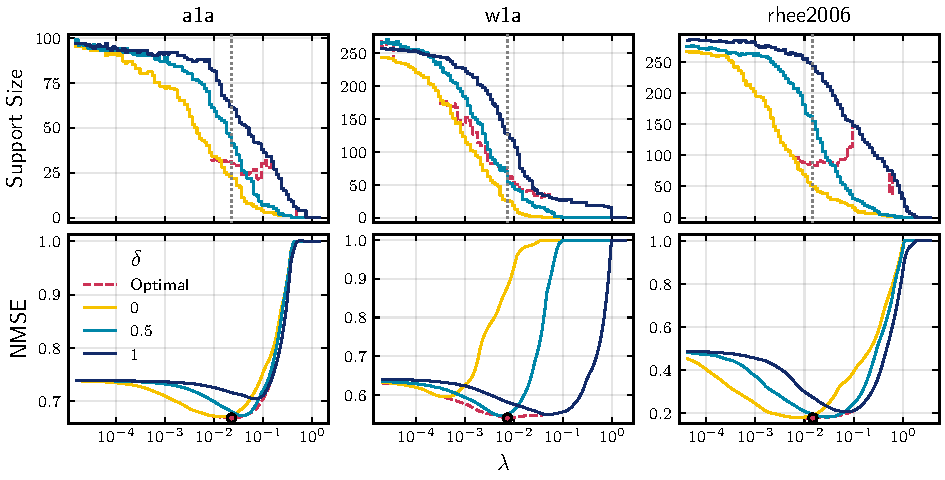
\includegraphics[]{plots/hyperopt_paths.pdf}
  \caption{%
    Support size and normalized mean-squared error (NMSE) for the validation set for the lasso fit to datasets \data{a1a}, \data{w1a}, and \data{rhee2006} across combinations of \(\delta\) and \(\lambda\). The optimal \(\delta\) is marked with dashed black lines and the best combination of \(\delta\) (among 0, 1/2, and 1) and \(\lambda\) is shown as a dot.
  }
  \label{fig:hyperopt-support}
\end{figure}

\subsection{Mixed Data}\label{sec:experiments-mixed-data}

In \Cref{sec:mixed-data}, we discovered that extra care needs to be taken when normalizing mixed data. In this experiment, we construct a quasi-normal feature with mean zero and standard deviation 1/2 and a binary feature with varying class balance \(q\). We set the signal-to-noise ratio to 0.5 and generate our response vector \(\vec{y}\) as before, with \(n = \num{1000}\). These features are constructed so that their effects are comparable under the notion of comparability that we introduce in \Cref{sec:mixed-data}, using \(\kappa = 2\). In order to preserve the comparability for the baseline case \(q_0 = 1/2\), we use the scaling introduced in \Cref{sec:mixed-data}, which leads to \(s_j = 2 \times (1/4)^{1-\delta}(q-q^2)^\delta\).
For the lasso, we set the level of penalization to

The results~(\Cref{fig:lasso-ridge-comparison}) reflect our theoretical results from \Cref{sec:theory}. In the case of the lasso, we need \(\delta =1\) to avoid the effect of class imbalance, whereas for ridge we instead need \(\delta =1/2\) (standardization). As our theory suggests, this extra scaling mitigates this class-balance dependency at the cost of added variance.

\begin{figure}[htpb]
  \centering
  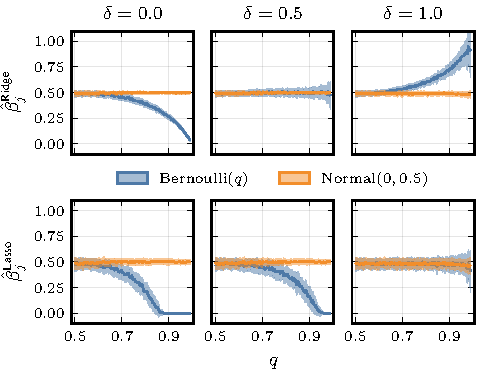
\includegraphics{plots/mixed_data.pdf}
  \caption{%
    Lasso and ridge estimates for a two-dimensional problem where one feature is a binary feature with class balance \(q\), \(\bernoulli(q)\), and the other is a quasi-normal feature with standard deviation 1/2, \(\normal(0, 0.5)\). Here, we have \(n = \num{1000}\) observations. The signal-to-noise ratio is 0.5 In every case, we standardize the normal feature. The binary feature, meanwhile, is centered by its mean and scaled by \((q-q^2)^\delta\). The experiment is run for 50 iterations and we aggregate and report means and standard deviations of the estimates.}
  % TODO: fix scaling parameterizaiton here. we are adjust to put features on even footing.
  \label{fig:lasso-ridge-comparison}
\end{figure}

Note that we do not see the bias reduction that we observed in our theoretical results for high \(q\) values and \(\delta \geq 1/2\) in \Cref{fig:lasso-ridge-comparison}. This is related to the error term (signal-to-noise ratio) and level of \(q\). Typically, we would need stronger class imbalance and larger error for the effect to show up in our experiments.

\subsection{Interactions}\label{sec:experiments-interactions}

In our final experiment, we study the effect of normalization and class balance on interactions when using the lasso. Our example consists of a two-feature problem with an added interaction term given by \(x_{i3} = x_{i1}x_{i2}\). The first feature is binary with class balance \(q=0.9\) and the second quasi-normal with standard deviation 0.5. We set \(n=1000\). Note that we perform normalization \emph{after} the interaction term is added.

The results~(\Cref{fig:interactions}) show, as before, that class balance (which, recall, is set to 0.9 here) has a dramatic effect on estimates of the binary feature when \(\delta \in \{0, 1/2\}\). Somewhat surprisingly, however, the interaction term does not seem to be affected by the normalization type for any of the cases in which it is present.

\begin{figure}[htpb]
  \label{fig:interactions}
  \centering
  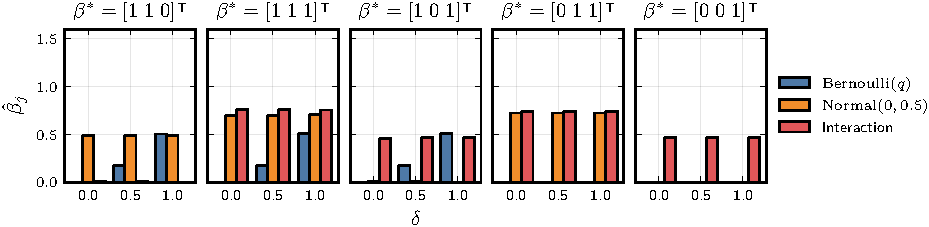
\includegraphics[]{plots/interactions.pdf}
  \caption{%
    Lasso estimates for a three-feature problem where the third feature is an interaction term between the first two features. The first feature is binary with class balance \(q=0.9\) and the second is quasi-normal with standard deviation 0.5. The signal-to-noise ratio is 0.5. The experiment is run for 50 iterations and we aggregate and report means across all iterations.
  }
\end{figure}

Note that the interaction in this experiment naturally introduces correlation between the features and that this has an effect on the lasso estimates since we, for instance, can penalize the main effect whilst still retaining information about it in the interaction term.


